% Chapter Template

\chapter{A Primer on Artifical Neural Networks} % Main chapter title

\label{Chapter3} % Change X to a consecutive number; for referencing this chapter elsewhere, use \ref{ChapterX}

\lhead{Chapter 3. \emph{A Primer on Artifical Neural Networks}} % Change X to a consecutive number; this is for the header on each page - perhaps a shortened title

%----------------------------------------------------------------------------------------
%	SECTION 1
%----------------------------------------------------------------------------------------
\section{Introduction}
This chapter presents an overview of the mathematical theory behind artificial neural networks and how they learn. It should serve as a quick guide to the techniques used in the experiments within this thesis.

\section{Perceptrons}
\label{sec:percep}
The perceptron is the parent of modern artificial neurons \cite{rosenblatt1958perceptron}.
Perceptrons arranged in layers, referred to as multi-layer perceptrons, are therfore the predecessor of modern artificial neural networks.

\subsection{What is a Perceptron}



\begin{figure}
	\centering
	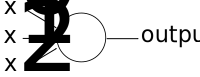
\includegraphics[width=0.5\textwidth]{Figs/intro2dl/perceptron.png}
	
	\caption{A perceptron with three binary inputs, $x_0, x_1, x_2$.}
	\label{fig:perceptron}
\end{figure}

Perceptrons are biologically inspired computation units and are a type of artificial neuron. They take a series of binary inputs, compute a weighted sum and produce a binary output based on the value of this sum as seen in figure \ref{fig:perceptron}.


\begin{equation}
output = \begin{cases}
0 &\text{if $\sum_{j} w_j x_j + b < 0$}\\
1 &\text{if $\sum_{j} w_j x_j + b \geq 0$}
\end{cases}
\label{eqn:percep} 
\end{equation}

Where $x_j$ is the jth input, $w_j$ is it associated weight and $b$ is a constant value called the bias, which affects how easy it is for the neuron to activate. The output of the perceptron is caluclated using the formulation shown in \ref{eqn:percep}.

By adjusting each of the weights we can change the output of the perceptron. For example, if we wanted to use a perceptron to decide whether to have a picnic today we can  select a set of relevant inputs, ``the weather is nice" and ``the pollen count is low".

If it is a sunny day, and the pollen count is high, the input to the perceptron would be $[1,0]$.
 
We will set our weights depending on how important each of the inputs is. No one likes a picnic in the rain, so the weather is important, whilst the pollen count is only important if you suffer from hayfever. We will select a bias of -5 for our perceptron.

For person A, the weights might look like $[7, 0]$ (person A doesn't suffer from hayfever). Therefore the output of the perceptron would be 1 as $1 \times 7 + 0 \times 0 - 5 = 2$ is greater than 0, so person A will go for a picnic.

Person B owns a large umbrella (so the weather doesn't matter as much) but they do suffer from hayfever, their weights might look like $[4, 7]$. The output of the perceptron would be 0 as  $1 \times 4 + 0 \times 7 - 5 = -1$ is less than 0. Therefore, person B would wait for a day with a lower pollen count for a picnic.


\subsection{Multi-Layer Perceptron}
In the previous section I demonstrated how a single perceptron can be used to make decisions based on a set of inputs. However, things get much more interesting when we start to link multiple perceptrons together into multi-layer perceptrons (MLP).

\begin{figure}
	\centering
	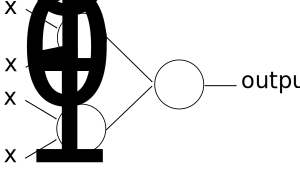
\includegraphics[width=0.5\textwidth]{Figs/intro2dl/mlp.png}
	
	\caption{A multi-layer perceptron consisting of three perceptrons arranged in two layers, with three binary inputs, $x_0, x_1, x_2$.}
	\label{fig:mlp}
\end{figure}

If we take the example from the previous section about deciding to go for a picnic or not, we can use the MLP shown in \ref{fig:mlp} to consider what happens if person A and B want to go for a picnic together.

Given the previous conditions of a sunny day with a high pollen count, person A wants to go whilst person B does not, as demonstrated by the outputs of their individual perceptrons. Taking these outputs as inputs to the second layer of our MLP, we can see whether the picnic will go ahead.

This time we will set the weights of the second layer based on who shouts the loudest. In this case, person A really wants to go and is very vocal about it. $1 \times 9 + 0 \times 5 - 5 = 4$ so the picnic will go ahead. This resulted in person B developing a headache and sneezing a lot. Clearly we need to find a way to adjust the weights of our MLP so that it makes better decisions in the future.

\section{Activation Functions}

Only being able to handle binary values is a major drawback of the perceptron. An artificial neuron which can handle continuous values is much more useful.

This limitation occurs due to the activation function of the perceptron shown in equation \ref{eqn:percep}. Visualising the perceptron activation function highlights that changes in the output of the neuron are not proportional to changes in the weights of the neuron as seen in figure \ref{fig:activation_percep}. With a few small changes we can make an artifical neuron that accepts continuous values and has a continuous output.

\begin{figure}
\begin{center}
\begin{tikzpicture}

% Us


\begin{axis}[
axis lines=middle,
xtick={-10,0,10},
xticklabels={$-\infty$, 0, $\infty$},
xlabel={$\sum_{j} w_j x_j + b$},
ylabel={Output},
xlabel near ticks,
ylabel near ticks]
\addplot +[blue, thick, mark=none] coordinates{(-10,0) (0,0) (0,1) (10,1)};

\end{axis}

\end{tikzpicture}
\caption{Visualisation of the perceptron activation function.}
\label{fig:activation_percep}
\end{center}
\end{figure}

A continuous output is very important as it means that a small change in the weights of a neuron will cause a small change in its output. This makes it much easier to understand how changing the weights affects the output of the network as the change in output becomes proportional to the change in weights as shown in equation \ref{eqn:proport}

\begin{equation}
	\delta Output \propto \delta W
	\label{eqn:proport}
\end{equation}  


\subsection{Sigmoid Neurons}

The sigmoid neuron uses the sigmoid function, shown in equation \ref{eqn:sig} as its activation function. 

\begin{equation}
\sigma(z) = \frac{1}{1 + e^{-z}}
\label{eqn:sig}
\end{equation}

$z$ is the sum of the weights multiplied by their respective inputs as seen in equation  \ref{eqn:z_act}.

\begin{equation}
z = \sum_{j} w_j x_j + b
\label{eqn:z_act}
\end{equation}

As we can see in figure \ref{fig:activation_sigmoid}, as $z$ changes, their is a proportional change in the output $\sigma(z)$, unlike in figure \ref{fig:activation_percep} where the output only changes when $z$ crosses the y-axis.

\begin{figure}
\begin{center}
\begin{tikzpicture}



\begin{axis}[
axis lines=middle,
xtick={-10,0,10},
xticklabels={$-\infty$, 0, $\infty$},
xlabel={z},
ylabel={$\sigma$(z)},
xlabel near ticks,
ylabel near ticks]
\addplot[blue, thick, smooth, samples=1000, domain=-10:10]{1 / (1 + e^-x)};

\end{axis}
    

\end{tikzpicture}
\caption{Visualisation of the sigmoid activation function.}
\label{fig:activation_sigmoid}
\end{center}
\end{figure}

Now that we have an activation function that can produce continuous values, we can consider a much more diverse range of data to train our neural networks with. So instead of just making yes or no decisions we can look at, for example, the colours of pixels and decide if there is a cat in the image or given todays weather, predict if it will rain tomorrow.

\subsubsection{Other activation functions}
There are two other important and commonly used activation functions, though many others exist. These are, the hyperbolic tangent (Tanh) shown in figure \ref{fig:activation_tanh} and rectified linear unit (Relu)  shown in figure \ref{fig:activation_relu}.

\begin{figure}[h]
\begin{center}
\begin{tikzpicture}
\begin{axis}[
axis lines=middle,
xtick={-10,0,10},
xticklabels={$-\infty$, 0, $\infty$},
xlabel={z},
ylabel={$\sigma$(z)},
xlabel near ticks,
ylabel near ticks]
\addplot[blue, thick, smooth, samples=100, domain=-10:10]{tanh(x)};

\end{axis}
    

\end{tikzpicture}
\caption{Visualisation of the hyperbolic tangent activation function.}
\label{fig:activation_tanh}
\end{center}
\end{figure}

The Tanh function looks similar to the sigmoid function, however it has an output between negative one and one, where the sigmoid goes from zero to one. This is useful when having negative values within the network is important.

\begin{figure}[h]
\begin{center}
\begin{tikzpicture}
\begin{axis}[
axis lines=middle,
xtick={-10,0,10},
xticklabels={$-\infty$, 0, $\infty$},
xlabel={z},
ylabel={$\sigma$(z)},
xlabel near ticks,
ylabel near ticks]
\addplot[blue, thick, smooth, samples=1000, domain=0:10]{x};
\addplot[blue, thick, smooth, samples=1000, domain=-10:0]{0};

\end{axis}
    

\end{tikzpicture}
\caption{Visualisation of the rectified linear unit activation function.}
\label{fig:activation_relu}
\end{center}
\end{figure}

The Relu was created to address and issue known as vanishing gradients. This is to do with how neural networks are trained, as expalined in the enxt session. Briefly, as training depends on error gradients, having a linear activation function means that deeper networks \footnote{Deeper networks are beneficial as they can make more complex decisions by layering more and more simple decsions as shown in the MLP example in section\ref{sec:percep}} can be trained as non-linear functions like the sigmoid or Tanh will have reduced gradient magnitude when they are differentiated to backpropogate the error through the network. If that doesn't make sense yet, don't worry, it will become clear shortly.

\section{Learning Algorithms}
In section \ref{sec:percep} we saw how simple computation units can make simple decisions and how these can be chained together to make more complex decisions. However, sometimes the decisions we make are wrong and we need to learn from our mistakes.

In general, perceptrons (and their more modern decendents) will have their initial weights set randomly, unlike in our example where I chose them. 

Randomly setting weights is useful in practice as we will usually have large numbers of inputs, weights, layers and artifical neurons, so setting each by hand would be intractable. Also, if we knew what weights to set, we wouldn't need a neural network or a learning algorithm to solve our problem as we would likely have a more efficient mathematical description of the problem \footnote{there is a large body of work concerning the best way to initialise neural networks, I will briefly comment on this in section \ref{sec:random_init}.} 

With random weights our networks will make a lot of wrong decisions! However if we have a smart way of adjusting our weights we can make our neural networks get better at making decisions over time. This improvement is what I am referring to when I say ``machine learning''.

\subsection{Types of Training}
There are many ways to train neural networks, supervised, unsupervised, reinforcement or 
adversarial learning (to name a few). The experiments in this thesis will focus on supervised and unsupervised learning. %However, here is a brief description of the more prominant methods.


\textbf{Supervised learning} - an external system is used to provide ground truth values for the desired output of the network. An example would be classification using standardised datasets like MNIST handwritten digits \cite{lecun1998mnist}.


\textbf{Unsupervised learning} - no external system provides ground truth values, instead these are inferred directly from the data. Autoencoders (discussed in great deal in later chapters) are a good example of this.  

%\todo[inline]{finish this}
%\textbf{Reinforcement learning} - an external system provides a score which estimates the value of an action (think about getting points in a video-game). Training a dog by giving it treats when it performs a trick is reinforcement learning. We reinforce the desired behaviour by rpoviding a reward.

%\textbf{Adversarial learning} - two networks are trained in tandom, a generator and a descriminator. The


\subsection{Cost functions: How wrong am I?}
In order for our neural networks to learn, they need feedback as to how wrong they are. This is done using a cost function, a formula which gives a measure of how good or bad our network is at a particular task.

Depending on the particular method we use to train our networks, the cost function may be given a different name. For example in reinforcement learning, the cost function is typically called a value function. However, they all serve the same purpose, which is to provide feedback as to how well our network is doing at the task it has been assigned. Therefore, to avoid jargon I will refer to this as a cost or loss function throughout this thesis.

The cost fuction can take on many forms, in supervised and unsupervised training alike. Here are a few of the more commonly used ones and an explanation of each.

\subsubsection{Mean Squared Error}
Mean squared error (MSE) measures the average difference between points as shown in equation \ref{eqn:mse}.

\begin{equation}
C = \frac{1}{n}\sum_{i=0}^{n} (Y_i - \hat{Y_i})^2
\label{eqn:mse}
\end{equation}

When used as a loss function, MSE gives a measure of how bad our estimate $\hat{Y_i}$ is of our true value $Y_i$ on average for for all $n$ training samples in a given dataset. A perfect model would have an MSE of 0 as $\hat{Y_i}$ would be equal to $Y_i$ for all values of $i$.

In general, $Y_i$ and $\hat{Y_i}$ can be of arbitrary size and shape (as long as they match each other). That is, they can be scalers, vectors or matricies.

\subsubsection{Cross-Entropy}
Cross-entropy measures the error between two probability distributions $P$ and $Q$ using the formula shown in equation \ref{eqn:xntrpy}. $P$ is the true probability distribution which we are trying to model with our predicted probability distribution $Q$.

\begin{equation}
C = -\sum_{i=0}^{n}P(i) log(Q(i))
\label{eqn:xentrpy}
\end{equation}

When using cross-entropy as a loss function, we can view the output of our neural network as a probability distribution. For example, in a multiclass classification problem with $k$ classes, each of the $k$ outputs of the network tells us the probability that the network believes an input to belong to class $k$.

Here is a more concrete example:
Given a dataset containing images of animals: cats, dogs, horses and snakes. A single image containing a cat would be labelled $[1, 0, 0, ..., 0]$. This tells us the exact probability distribution of the image, $P$ i.e. the image certainly contains a cat and does not contain any other animals.

now as our network trains, it may give a prediction of $[0.5, 0.3, 0.15, 0.05]$, this is our predicted probability distribution $Q$.

Calculating our cross-entropy we get:
\begin{equation}
C = -\sum_{i=0}^{n}P(i) log(Q(i))
\label{eqn:xentrpy_eg}
\end{equation}




\subsubsection{Kullback-Leibler Divergence}


\subsection{Gradient Decent}
now that we have a method for determining how well our neural network performs a task, we can observe how this changes as the weights of the network are changed.

\pgfplotsset{%
  colormap={whitered}{color(0cm)=(white);
  color(1cm)=(orange!75!red)}
}

\begin{figure}
\begin{center}
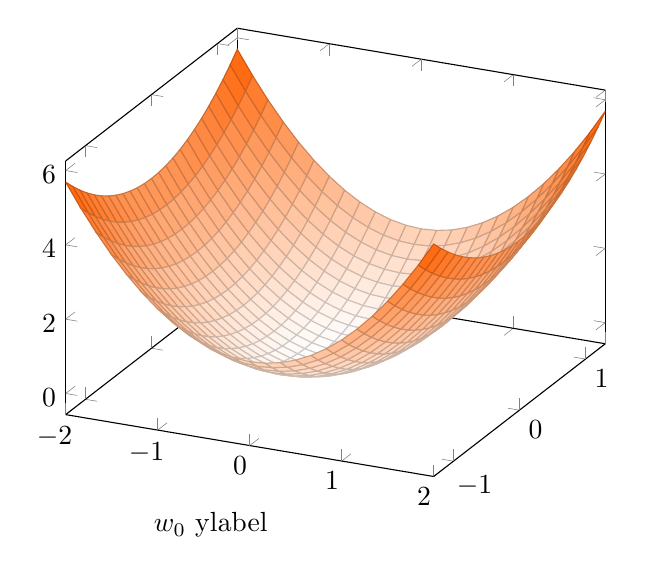
\begin{tikzpicture}
 
  \begin{axis}[
  xlabel = $w_0$
  ylabel = $w_1$
  ]
   
    \addplot3[
	surf,
	domain=-2:2,
	domain y=-1.3:1.3,
] 
	{x^2+y^2};

    
  \end{axis}
\end{tikzpicture}
\caption{The cost landscape of a bivariate function}
\label{fig:costscape}
\end{center}
\end{figure}

To make things simple, lets assume our network only has two weights, though the following derivation generalises to any number of weights. This could give us a cost landscape like that shown in figure \ref{fig:costscape}. Our aim is to minimise the cost as the cost is a measure of how wrong our network is.

In more definate terms we wish to minimise equation \ref{eqn:cost_bivar}, where $Y_i$ is the desired output value for input $i$ and $z$ is as defined in equation \ref{eqn:z_act}.

\begin{equation}
C(w_0, w_1) = \frac{1}{n}\sum_{i=0}^{n} (Y_i - \sigma(z_i))^2
\label{eqn:cost_bivar}
\end{equation}

This is the mean squared error rewritten slightly to highlight the dependence on the weights of the network.

If we make a small change to either of the weights $w_0$ and $w_1$ we will get a small change in the cost, $C$ as seen in equation \ref{eqn:delta_C}.

\begin{equation}
\Delta C \approx \frac{\delta C}{\delta w_0} \Delta w_0 + \frac{\delta C}{\delta w_1} \Delta w_1
\label{eqn:delta_C}
\end{equation}

We want to minimise C so we want $\Delta C$ to be negative. To make $\Delta C$ negative we will need to first denote that the gradient of $C$, $\nabla C$. 

\begin{equation}
\nabla C \equiv (\frac{\delta C}{\delta w_0}, \frac{\delta C}{\delta w_1})^T
\label{eqn:nabla_c}
\end{equation}

In equation \ref{eqn:nabla_c} we can see that the gradient of $C$ is equivalent to the partial derivatives of $C$ with repect to the weights of the network. For simplicity we will collect the changes in weights into a single vector $\Delta w \equiv (\Delta w_0, \Delta w_1)^T$.

By substituing this into equation \ref{eqn:delta_C} we get equation \ref{eqn:delta_c_sub}.

\begin{equation}
\Delta C \approx \nabla C \cdot \Delta w 
\label{eqn:delta_c_sub}
\end{equation}

Looking at equation \ref{eqn:delta_c_sub}, we can see that to make $\Delta C$ negative we can set $\Delta w$ as in equation \ref{eqn:delta_w_eta}, where $\eta$ is a small positive constant called the learning rate.

\begin{equation}
\Delta w = -\eta \nabla C
\label{eqn:delta_w_eta}
\end{equation}

By substituting equation \ref{eqn:delta_w_eta} into equation \ref{eqn:delta_c_sub} we can see that $ \Delta C = - \eta \abs{\nabla C}^2$ and because
 $\abs{\nabla C}^2 \geq 0$ this gaurantees that $C$ will always decrease if the weights are changed in accordance to equation \ref{eqn:delta_w_eta}.

By iteratively making changes to the weights according to \ref{eqn:delta_w_eta} we will eventually reach the minima of $C$ so long as we select an appropriate learning rate \footnote{Learning rate is discussed in more detail in section \ref{sec:lr_sch}}. 

\subsection{Backpropagation}
\subsection{Extensions and Improvements}
\subsubsection{Learning Rate Schedule}
\label{sec:lr_sch}
\subsubsection{Momentum}




\section{Convolutional Neural Networks}
\subsection{What is Convolution?}
\subsubsection{Kernels}
\subsubsection{Strides}
\subsubsection{Dilations}
\subsection{Transposed Convolutions}


\section{Recurrent Neural Networks}
\subsection{Vanilla RNN}
\subsection{Gated RNN}




\section{Summary}
